\documentclass[a4paper,12pt]{report}
\usepackage{amssymb,amsthm,amsmath,makeidx,verbatim,latexsym,amsfonts,graphicx}
%\renewcommand{\bibname}{References}
\newtheorem{Def}{Definition}[section]
\newtheorem{theorem}{Theorem}
\newtheorem{lemma}{Lemma}
 \numberwithin{equation}{section}
\linespread{1.3}
\pagenumbering{roman}
\begin{document}
%\thispagestyle{empty}
\begin{center}
\textbf{GLOBAL STABILITY ANALYSIS AND ITS APPLICATION IN DYNAMICAL SYSTEM}
\end{center}
\ \
\begin{center}
\text{BY}
\end{center}
\ \
\begin{center}
\text{AKOZI EMMANUEL OSHOHA}
\end{center}
\begin{center}
\textbf{Matric. number: 185600}
\end{center}
\begin{center}
\text{An undergraduate project in the Department of  Mathematics,}
\end{center}
\begin{center}
\text{Submitted to the Faculty of Science }  
\end{center}
\begin{center}
\text{in partial fulfilment of the requirement for the Degree of}
\end{center}
\begin{center}
\textbf{ BACHELOR OF SCIENCE}
\end{center}
\begin{center}
\textbf{of the}
\end{center}
\begin{center}
\textbf{UNIVERSITY OF IBADAN}
\end{center}
\begin{flushright}
\text{DECEMBER, 2018}
\end{flushright}
\addcontentsline{toc}{chapter}{Title Page}
\newpage
\addcontentsline{toc}{chapter}{Title Page}
\newpage
\section*{Certification} 
I certify that this project was carried out by {\bf ADENIYI EBENEZER OLAYINKA} in the department of Mathematics, University of Ibadan, Ibadan Nigeria.\\
\begin{center}
-----------------------------------------------\\
\textbf{Supervisor}\\
\textbf{O.B. Ogunfolu,}\\
\textbf{Department of Mathematics,}\\
\textbf{University of Ibadan, Nigeria} 
\end{center}
\addcontentsline{toc}{chapter}{Certification}
\newpage
\section*{Acknowledgements}
Adeniyi
\addcontentsline{toc}{chapter}{Acknowledgement}
\newpage
\section*{Dedication}
This thesis is dedicated to the glory of Almighty God, THE FATHER, THE SON and THE HOLY SPIRIT, who has made this programme a success.
\addcontentsline{toc}{chapter}{Dedication}
\newpage
\begin{center}
\section*{Abstract}
\end{center}
Adeniyi
\addcontentsline{toc}{chapter}{Abstract}
\newpage 
\addcontentsline{toc}{chapter}{Contents}
\tableofcontents
\newpage
\listoftables
\addcontentsline{toc}{chapter}{List of Tables}
\newpage
\listoffigures
\addcontentsline{toc}{chapter}{List of Figures}
\newpage
\pagenumbering{arabic}
\addcontentsline{toc}{chapter}{CHAPTER ONE}
\chapter{Introduction}
A dynamical system is a system whose state evolves with time over a state space according to a fixed rule. In creating a dynamical system one need to consider
(1) what is the 'SOMETHING' that will evolves over time.  (2) what is the rule that specifies how that 'SOMETHING'  evolves with time. In this way , a dynamical system is simply a model describing the temporal evolution of a system.

The state space is crucial to a dynamical system. A set of variables that give a complete description of the system at any particular time is necessary in the mathematical formulation of a dynamical system, these set of variables is called THE STATE VARIABLE also the set of all possible values of the state variables is called THE STATE SPACE. Dynamical system can be divided into two branches which are Discrete Dynamical System and Continuous Dynamical System. The discrete dynamical system is a dynamical system whose state evolves over state space in discrete time steps according to a fixed rule while the continuous dynamical system is one whose state evolves over state space continuously over time according to a fixed rule. The continuous dynamical system is the area of concentration in this text.


In dynamical system , a question to ask is that what will happen to the system with  time if the system is disturb, stability theory is the mathematical approach in understanding this theoretically. After which the system is been modelled into mathematical equation, It is easier to study the stability of the system. There are various type of stability which one can consider when studying how the system will react to disturbance which are linear stability, Lyapunov stability, orbital stability, structural stability, Von Neumann stability, hyper-stability e.t.c. and they fall under either local stability or global stability. The most important of them is the Lyapunov stability which can be characterized under local or global stability due to property of how the solution of the system behaves with one or more initial points which will be implore in understanding the stability of dynamical system in this text. In analysing   
the stability of a dynamical system using the Lyapunov stability the Lyaponov function is used. The main difficulty that one can encounter is the construction of the Lyaponov function which in general has no rules for construction.The existence of lypunov function is a necessary and sufficient condition for stability
\section{Stability Problem}
In 1944, the formal soviet unions scholar and control expert, A.I. Lurie, based on the study of many practical control systems including aircraft automatic control proposed the following non-linear control system
 \begin{equation} \left.
 \begin{array}{lllll}
 \frac{dx}{dy} &=& Ax + f( \sigma)\\ 
\sigma &=& c^T x
\end{array} \right\}
\end{equation} 
where $ x\in \mathbb{R}^n, \ b,c \in \mathbb{R}^n, \ A \in \mathbb{R}^{n \times n}, \ and \ f( \sigma ) > 0\ where \ \sigma \neq 0 $
Lurie developed a method to deal with the stability of the non-linear control system (1.1) which he called non-linear isolation method. The non-linear part of the system is isolated so that the system becomes one with closed- loop form.\\
A more general mathematical description of a dynamical system can be given by a finite set of n-quantities $ X_1,X_2,X_3,..., X_n $ whose the rate at which they change with time is given as follows:
\begin{equation} \left.
\begin{array}{lllll}
\frac{dX_1}{dt} &=& F_1(X_1, X_2,..., X_n, t)\\
\frac{dX_2}{dt} &=& F_2(X_1, X_2,..., X_n, t)\\
\vdots \\
\frac{dX_n}{dt} &=& F_n(X_1, X_2,..., X_n,t)
\end{array} \right\}
\end{equation}
A little change in notation can occur using the notation
\begin{equation*}
\frac{dX_i}{dt} = \dot{X_i}
\end{equation*}
The equation can also be written as:
\begin{equation}
\frac{dX}{dt} = F(t, x(t))
\end{equation}
such that
\[\textbf{X}=\begin{pmatrix}
x_{1}\\
x_{2}\\
\vdots\\
x_{n}
\end{pmatrix}\quad\text{and}\quad {\bf F(t,x(t))}=\begin{pmatrix}
F_1(X_1, X_2,..., X_n, t)
\\ F_2(X_1, X_2,..., X_n, t)
\\ \vdots
 \\ F_n(X_1, X_2,..., X_n,t)
\end{pmatrix}.\] \\
with, \\
$X: \mathbb{R}\longrightarrow \mathbb{R}^n$ \\ 
$F:\mathbb{R} \times \mathbb{R}^n \longrightarrow \mathbb{R}^n$ \\
REMARKS\\
(1)The differential equations are ordinary, there are no partial derivatives \\
(2)They are of the first order. If higher order derivatives appears, it can always be reformulated into a system of first order ordinary differential equations. \\
(3)Given the system of ordinary differential equation (1.1.3) \\
\begin{equation}
\frac{dX}{dt}= F(t,X(t)) \ and \ X(t_o)=X_o
\end{equation} \\
The existence and uniqueness of the solution of the system can be proved by using a suitable theorem for showing the existence and uniqueness of the solution. \\
(4) A system of equation is called AUTONOMOUS SYSTEM if (1.13) is of the form 
 \begin{equation}
 \frac{dX}{dt}=F(X(t))
 \end{equation}
 The stability studies of (1.13) will be provided in chapter 2 \\
 The Lyapunov functions which is the core in studying the lyapunov stability of a dynamical system will be examine in chapter two with the lyapunov stability theorem. \\
In dynamical system, at the long run, as the system changes with time, the goal is to study and analysed the system when small perturbation affects the system. To study the stability of the system of differential equation \\
\begin{equation*}
\frac{dX}{dt}=F(t,X(t))
\end{equation*}
 The equilibrium points of the system is given as the points $x \in \mathbb{R}^n$ which make 
 \begin{equation*}
 F(t,X(t))= 0
\end{equation*} \\
More analysis can be done when the equilibrium points of the system is known, equilibrium points serves as a majoy key in understanding the stability of the system 
\section{System of differential equations}
A differential equation is a mathematical equation that relates a function with its derivatives. This equation plays a prominent role in many disciplines including engineering, physics, economics and biology.


Differential equation first came into existence with the invention of calculus by Isaac Newton and Gottfried Wilhelm (Von) leibniz. Isaac newton listed three kinds of differential equation
\begin{equation*}
\frac{dy}{dx}=f(x)
\end{equation*} 
\begin{equation*}
\frac{dy}{dx}=f(x,y)
\end{equation*}
\begin{equation*}
x_1\frac{\partial y}{\partial x_1}+ x_2\frac{\partial y}{\partial x_2}=y
\end{equation*}
which he solves using infinite series and also discusses the non-uniqueness of solutions.

In the year 1695 Jacob Bernoulli proposed the Bernoulli differential equation which is of the form
\begin{equation*}
y^\prime+p(x)y=Q(x)y^n
\end{equation*}
for which the following year Leibniz obtained solutions by simplifying it. Ever since the topic 'differential equation' has been expanding. When the function in consideration depends on one independent variable then the differential equation is called 'Ordinary Differential Equation' and when the function depends on two or more independent variable then the differential equation is called 'Partial Differential equation'. The linearity, non-linearity and homogeneity, non-homogeneity of the types of differential equations can be considered with their respective solutions.

System of differential equation is used in the modelling of the behaviour of a dynamical system . In this text linear system of ordinary differential equations will be considered
\subsection*{Linear system} A linear system is a system of differential equations of the form 
\begin{equation} \left.
\begin{array}{lllll}
X_{1}^\prime &=& a_{11}X_{1}+ ...+ a_{1n}X_{n}+F_{1} \\
X_{2}^\prime &=& a_{21}X_{1}+ ...+ a_{2n}X_{n}+F_{2}\\
\vdots \\
X_{n}^\prime &=& a_{n1}X_{1}+ ...+ a_{nn}X_{n}+F_{n}
\end{array} \right\}
\end{equation}
where $ \prime = \frac{d}{dt} $.
Given that $ A_{ij}(t) \ and \ F_{j}(t) $
are functions on the interval $ a<t<b \ with \ a,b \in \mathbb{R}, \ X_{1}(t),X_{2}(t),...,X_{n}(t) $ is the unknown functions.\\
The system is called homogeneous if all $ F_{j} ' s = 0 $, otherwise it is called non-homogeneous.
\subsubsection*{Matrix notation}
A non-homogeneous system of linear equations of the form (1.2.1) is written as the equivalent to the vector-matrix system
\begin{equation}
X^\prime(t)=A(t)X(t)+F(t)
\end{equation}
\[\textbf{X(t)}=\begin{pmatrix}
x_{1}(t)\\
x_{2}(t)\\
\vdots\\
x_{n}(t)
\end{pmatrix}\quad , \textbf{F(t)}=\begin{pmatrix}
F_{1}(t) \\
F_{2}(t) \\
\vdots \\
F_{n}(t)
\end{pmatrix} \text{and}\quad {\bf A(t)}= \left( \begin{matrix}
a_{11} \ a_{12} \ ... \ a_{1n} \\
a_{21} \ a _{22} \ ... \ a_{2n} \\  
\vdots \qquad \vdots \qquad \vdots \\
a_{n1} \ a_{n2} \ ... \ a_{nn}
\end{matrix} \right) \]
Note: since the highest derivative of (1.2.1) is 1 and the unknown function depends on one independent variable, the system of differential equation takes the name 'system of n-first order ordinary differential equation' \\
\section{Methods of solving linear system of first order ordinary differential equation with constant coefficient}
How to get solutions for linear system of first order ordinary differential equations of the form of (1.2.2) will be discuss here
\subsection{Homogeneous linear system}
The linear system of the form (1.2.2) is said to be homogeneous if F(t)=0, which reduces the equation to 
\begin{equation}
X^\prime=A(t)X(t)
\end{equation} 
the problem of how to solve the above equation is of interest. \\
The equation (1.3.1) can be solve by the following methods \\
\subsubsection*{\textbf{Triangular Method} }
Considering a system of 2-first order ordinary equation of the form 
\[ \begin{pmatrix}
X_{1} \\
X_{2}
\end{pmatrix}^\prime = \left( \begin{matrix}
a \quad b \\
c \quad d
\end{matrix} \right) \begin{pmatrix}
X_1 \\
X_2
\end{pmatrix} \]
when b=0, then the matrix reduces to a triangular matrix,then it can be rewritten as 
\begin{equation*}
X_{1}^\prime=aX_{1} 
\end{equation*}
\begin{equation*}
X_{2}^\prime=cX_{1}+dX_{2}
\end{equation*}
the first equation can be solve by separation of variable which yield the solution
\begin{equation*}
X_{1} = X_{0} \exp at
\end{equation*}
if this is inserted into the second equation, the second equation reduces to 
\begin{equation*}
X_{2}= dX_{2}+cX_{0}\exp at
\end{equation*}
the reduced form is a linear first order equation of the form
\begin{equation*}
Y^\prime=P(t)Y+Q(t)
\end{equation*}
and can by solved by the integrating factor method which gives the required second solution. This can be extended to system of n-first order differential equation if the matrix A(t) is a triangular matrix by solving it recursively. \\
\subsubsection*{\textbf{Non-Triangular method} }
This is a general method for solving system of first order ordinary differential equation which involves the use of eigenvalue and eigenfunction of the matrix A(t) in (1.3.1). Given that  
\begin{equation*}
X^\prime(t)=AX(t)
\end{equation*}
where \textbf{A} is real, n$\times$n constant matrix. As solution, one will try 
\begin{equation}
X^\prime=C e^{rt}
\end{equation}
where C is a constant vector. Then 
\begin{equation}
X^\prime=rCe^{rt}
\end{equation}
Then we have a solution provided that
\begin{equation*}
rCe^{rt}=ACe^{rt} \quad then \quad (A-rI)C=0
\end{equation*}
and for non-trivial solution(i.e a $\neq $0), r must satisfy
\begin{equation}
|A-rI|=0
\end{equation}
\subsubsection*{Procedure}
Finding eigenvalues, $r_{1},r_{2,...,r_{n}}$, solution of $|A-rI|=0$ and the corresponding eigenvectors, $a_{1},a_{2},a_{3},...,a_{n}$. Then if the n eigenvectors are linearly independent, we have a general solution
\begin{equation}
X=a_{1}C_{1}e^{r_{1}t}+a_{2}C_{2}e^{r_{2}t}+ ... + a_{n}C_{n}e^{r_{n}t}
\end{equation}
where $a_{1},a_{2},a_{3},...,a_{n}$ are arbitrary constants and also linearly independent
\subsubsection*{Example}
\begin{equation*}
X^{\prime}=\left(\begin{matrix}
1 & 1 \\
4 & 1 
\end{matrix} \right)X
\end{equation*}
Consider $ X = Ce^{rt}$. Then we require 
\begin{equation*}
(A-rI)\begin{pmatrix}
a_{11} \\
a_{21}
\end{pmatrix}=\begin{pmatrix}
0 \\
0
\end{pmatrix}
\end{equation*}
\begin{equation*}
|A-rI|=\left| \begin{matrix}
1-r & 1 \\
4 & 1-r
\end{matrix} \right|=0
\end{equation*}
\begin{equation*}
(1-r)^{2}-4=0 \Rightarrow (1a-r)^{2}=\pm 2
\end{equation*}
r=3,-1. So the eigenvalues are 3 and -1 \\
with r=3
\begin{equation*}
\left(\begin{matrix}
-2 & 1 \\
4 & -2
\end{matrix}\right) \begin{pmatrix}
a{1} \\
a_{2}
\end{pmatrix}=\begin{pmatrix}
0 \\
0
\end{pmatrix}
\end{equation*}
So $ -2c_{1}+c_{2}=0 $ implies that $c_1 =1$ and $ c_{2}=2$. Hence, the eigenvector will be 
\begin{equation*}
\begin{pmatrix}
1 \\
2
\end{pmatrix}
\end{equation*}
with $r = -1$
\begin{equation*}
\left(\begin{matrix}
2 & 1\\
4 & 2
\end{matrix}\right) \begin{pmatrix}
a_{1} \\
a_{2}
\end{pmatrix}=\begin{pmatrix}
0 \\
0
\end{pmatrix} 
\end{equation*}
 So $ 2a_{1}+a_{2}=0 $ implies that $ a_{1}=1 \ and \ a_{2}=-2$. Therefore, the eigenvector will be 
 \begin{equation*}
 \begin{pmatrix}
 1 \\ 
 -2
 \end{pmatrix}
 \end{equation*}
 The general solution is
 \begin{equation}
 X = a_{1}\begin{pmatrix}
 1 \\
 2
 \end{pmatrix}e^{3t}+a_{2}\begin{pmatrix}
 1 \\
 -2
 \end{pmatrix}e^{-t}
 \end{equation}
 The equation (1.3.6) is a family of solutions since $a_{1} \ and \ a_{2}$ are arbitrary (i.e., if $X_{1} \ and \ X_{2} \ are \ known \ at \  t \ = \ 0, $ we can solve (1.3.6) to get $a_{1} \ and \ a_{2}$ for specific solutions).\\
In general,solving the system make lead to the following possibility which can be solved by little extension of the usual method \\
1. If \textbf{A} is hermitian (i.e $\textbf{A} ^{T}$=$\overline{\textbf{A}}^{T}$=$\textbf{A}$, where $\overline{\textbf{A}}$ is the conjugate of the matrix), then the eigenvalues are real and can be find n linearly-independent eigenvectors. \\
2. $\textbf{A}$ is non-hermitian. We  have the following possibilities \\
(a) n real and distinct eigenvalues and n independent eigenvectors \\
(b)Complex eigenvalues \\
(c)Repeated eigenvalues.
\subsection{Non-homogeneous systems}
We have 
\begin{equation}
X^\prime(t)=A(t)X(t)+F(t)
\end{equation}
We assume that we have solve $X^\prime=AX$. We actually have a procedure for A, a constant matrix. \\
\subsubsection*{(1)} If A has  n independent eigenvectors, the procedure is to build the matrix T with eigenvectors of A:
\begin{equation}
\textbf{T} = (a_{1} \ a_{2} \ a_{3} \ ... a_{n}\ )
\end{equation}
Then, we change variables X = Ty with $X^\prime = Ty^{\prime}$. Going back to the system 
\begin{equation}
X^{\prime} = T y^{\prime} = AX + F(t) = ATy+F
\end{equation}
As T is built with n eigenvectors, this is a regular matrix ( $\det T \neq 0$ ), so we can work out $T^{-1}$, the inverse of T. Hence, from (1.3.8)
\begin{equation}
y^{\prime} = T^{-1}ATy + T^{-1}F = Dy + H
\end{equation}
where D is the diagonal matrix of the eigenvalues of A. Therefore,
\begin{equation}
y^{\prime}_{i}(t)= r_{i} y_{i} (t) + H_{i}, \forall i = 1,2,...,n
\end{equation}
Hence
\begin{equation}
y_{i} = e^{r_{i}t} \int e^{-r_{i}t} H_{i} (t) dt + a_{i} e^{r_{i}t}, \forall i = 1,2,...,n
\end{equation}
After obtaining $ y _{i} $, we can get X = Ty.

This method is only possible if there are n linearly independent eigenvectors, i.e., A is diagonalizable constant matrix. Because we can reduce the matrix to its diagonal form, the above procedure works. In cases where we do not have the n independent eigenvectors, the matrix A can only be reduced to its Jordan canonical form.
\subsubsection*{(2) Variation of parameters}
Lets us consider the system (1.3.7), and we know the solution of the associated homogeneous system (1.3.5). The we can build the fundamental matrix of the system, $\Phi (t)$, whose columns are the linearly independent of the homogeneous system of solutions. We are looking for a solution like
\begin{equation}
X = \Phi (t) u(t)
\end{equation}
where u(t) is a vector to be determined such that (1.1.13) is a solution of (1.3.7). substituting
\begin{equation}
\Phi ^{\prime} (t) u(t) + \Phi (t) u^{\prime} (t) = A(t) \Phi (t) u(t) + F(t)
\end{equation} 
as we know that $ \Phi ^{\prime} (t) = A(t) \Phi (t) $,
\begin{equation}
\Phi (t)u(t) = F(t) \Longrightarrow u(t) \int \Phi ^{-1} (t)F(t)dt + C
\end{equation}
where C is a constant vector and there exists $ \Phi ^{-1} (t)$ since the n columns of matrix $\Phi (t)$ are linearly independent. The general solution is 
\begin{equation}
X(t) = \Phi (t) \int \Phi ^{-1} (t)F(t) dt 
+ C\Phi (t)
\end{equation}
\chapter{Stability Theory}
In this chapter, stability of dynamical system will be the main scope also with the mathematical tools used in studing them.

In the setting of dynamical system, stability is defined with respect to some given equilibrium points then one can say that a dynamical system is stable if it is stable at the equilibrium point. An equilibrium point is stable if when the state vector is moved slightly away from that point, it tends to return to it or at least does not keep moving further away. 

Stability theory addresses the stability of solutions of differential equations and of trajectories of dynamical systems under small perturbation of initial conditions. In this chapter, the linear and non-linear stability of dynamical system will be considered but before that the following definition is important.
\section*{Stability Definitions}
Let $ X^* $ be an equilibrium point of $ \frac{dX}{dt}= F(X)$ (i.e $ F(X^* )= 0$) and $X(t_0)$=X(0) an initial condition then $X^*$ is \\
(1) Locally stable, if for every $R>0$ there exists $r>0$ such that 
\begin{equation*}
|| X(0) - X^{*} ||<r(t_{0},R) \Longrightarrow || X(t) - X^* ||<R
 \  \forall t \geq t_0 \geq 0 
\end{equation*}  
(2) Locally asymptotically stable, if locally stable and 
\begin{equation*}
|| X(0)- X^*||<r \Longrightarrow \displaystyle{\lim t\to \infty} X(t)=X^* 
\end{equation*}
(3) Globally stable, if it stable for all X(0)$ \in \mathbb{R}^n$ \\
(4) Globally asymptotically stable, if it is asymptotically stable for all X(0)$\in \mathbb{R}$ \\
(5) Exponentially stable, if there are constants $\alpha,\delta,C >0$ such that 
\begin{equation}
||X(t)- X^*|| \leq Ce^{- \alpha t}|X - X(0)|, \ \ \forall | X - X|\leq \delta \ and \ t \ \geq t_0 \geq 0
\end{equation}
Clearly be exponentially stable implies stability as in one and global exponentially stability can be define in like manner as that of 3 and 4. \\
\textbf{Note}: The above definitions are all said to be uniformly stable if r is independent of $t_0$


First to consider in the stability theory is that of a linear dynamical system is that of the form 
\begin{equation} \frac{dX}{dt}=AX 
\end{equation}
where A is an invertible matrix. The equilibrium point is stable if and only if the eigenvalues of A at the equilibrium point are the following if the eigenvalues are \\\\
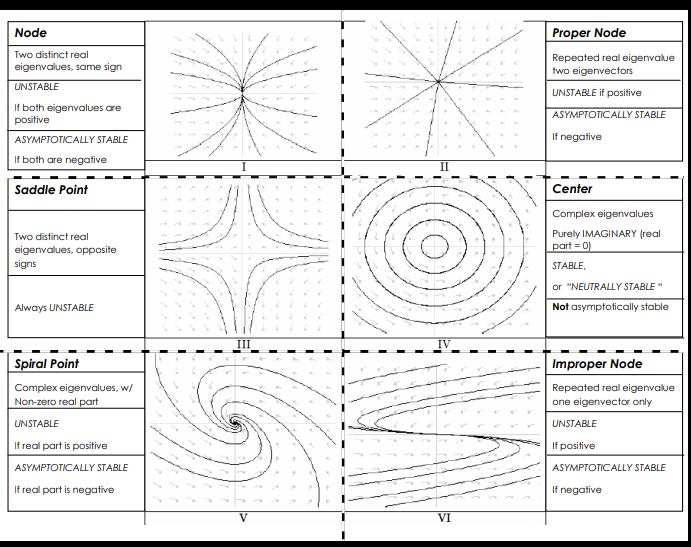
\includegraphics[scale=0.8]{1}

\theorem Given the system (2.0.2), where A is a constant matrix of order n then the following is true \\
(1) The equilibrium point x:=0 is stable if all the eigenvalues of the matrix A have only imaginary parts.\\
(2) If the eigenvalues all have negative real parts, then the trivial solution is asymptotically stable. \\
\textbf{Proof} \\
(1) If all the eigenvalues are imaginary then there exists a constant M>0 such that a fundamental matrix $\Phi (t)$ of the system with $\Phi(t_0)=I$, one have $\| \Phi (t)\| \leq M$. \\
Therefore any solution x(t) of the system whenever $\|x_{t_0}\| < \delta$ , then \\
\begin{equation*}
\|x(t)\| = \|x_{0}\Phi (t)\| \leq \|x_{0}\|M <\delta M < \epsilon 
\end{equation*}
With $\delta = \frac{\epsilon}{M}$, which shows that the equilibrium point is stable. \\
(2) Since the eigenvalues of the system have negative real part, there exists $\alpha,M >0$ such that 
\begin{equation*}
\|\Phi(t)\| \leq Me^{-\alpha(t-t_{0})} , t\geq t_{o}
\end{equation*}
Where $\Phi$ is the principal fundamental matrix for the system of equation.\\
Let $$ X_{T_{0}}=  X_{0} $$, then whenever $$ \| x_{t_0} \|= \| x_{0} \| \leq \delta $$ \\
one have 
\begin{equation*}
\|x(t)\|=\|x_{0}\Phi (t)\| \leq \|x_0\|\|\phi (t)\| \leq \|x_{0}\| Me^{-(t-t_0)} \leq \delta M <\epsilon 
\end{equation*}
For $\delta = \frac{\epsilon}{M}$, which gives it stability. \\
To establish that of asymptotic stability, then 
\begin{equation*}
\lim_{t\to \infty}\|x_{t}\|=\|x_{0}\|M \lim_{t \to \infty}e^{-\alpha(t-t_o)}=0
\end{equation*} 
\textbf{Note} If one of the eigenvalues is positive real number then the system is unstable
\section{linear Stability for an Autonomous System}
Let $ \frac{dX}{dt}=F(X(t))$ be an autonomous system and $ X^*$ be an equilibrium point for the system. By taking a multi-variable Taylor expansion of F(x) about the equilibrium point then the system id reduced to 
\begin{equation}
\frac{dX}{dt}= F(X^*)+ \frac{\partial F}{\partial X}\displaystyle \mid_{X^*} (X-X^{*})+ . . . \ and \ since \ F(X^*)=0
\end{equation}
\begin{equation}
\frac{dX}{dt}= \frac{\partial F}{\partial X} \mid_{X^*} (X - X^*)+ . . . 
\end{equation}
The partial derivative in the above equation is to be interpreted as the Jacobian matrix. If the component of the state variable X are($x_{1}, x_{2}, x_{3},. . . , x_{n}$) and the components of F are $(f_{1},F_{2},f_{3},...,f_{n})$ then the Jacobian is given as 
\begin{equation}
\left[\begin{matrix}
\frac{\partial f_{1}}{\partial x_1} \quad \frac{\partial f_{1}}{\partial x_{2}} \quad \hdots  \frac{\partial f_{1}}{\partial x_{n}} \\
\frac{\partial f_{2}}{\partial x_1} \quad \frac{\partial f_{2}}{\partial x_{2}} \quad \hdots  \frac{\partial f_{2}}{\partial x_{n}} \\
\frac{\partial f_{3}}{\partial x_1} \quad \frac{\partial f_{3}}{\partial x_{2}} \quad \hdots  \frac{\partial f_{4}}{\partial x_{n}} \\
\vdots \ \ \qquad \ \ \vdots \qquad \ \ \vdots \\
\frac{\partial f_{n}}{\partial x_1} \quad \frac{\partial f_{n}}{\partial x_{2}} \quad \hdots  \frac{\partial f_{n}}{\partial x_{n}} \\
\end{matrix}\right]
\end{equation} 
Now by defining $\delta X=X-X^*$, taking derivative of this we get $\frac{d\delta X}{dx}= \frac{dX}{dt} $ if $ \delta X $ is small, then only the first tern in (2.1.3) is significant since the higher terms involves powers of small displacement from equilibrium. If we want to know how trajectories behave near the equilibrium point e.g whether they move toward or away from the equilibrium point, it should therefore be good enough to keep just this term. Then we have 
\begin{equation}
\frac{\delta X}{dX}= J^* \delta X
\end{equation}
where $ J^* $ is the Jacobian evaluated at the equilibrium point. The matrix $ J^*$  is a constant, so this is just a linear differential equation. According to the theory of linear differential equations, the solution can be written as a superposition of terms of the form $e^{\lambda _{i}t}$ where {$\lambda _{j} $} is the set of eigenvalues of the Jacobian.


The eigenvalues of the Jacobian are, in general, complex numbers. Let $\lambda_{i}=\mu _{i}+iv_{i}$, where $\mu _{i} \ and \ v_{i} $ are, respectively, the real and imaginary parts of the eigenvalue. Each of the exponential terms in the expansion can therefore be written as 
\begin{equation}
e^{\lambda _{i}t}=e^{\mu _{i}t}e^{iv_{i}t}
\end{equation}
The complex exponential in turn can be written as 
\begin{equation}
e^{iv_{i}t} = cos(v_{i}t)+isin(v_{i}t)
\end{equation}
The complex part of the eigenvalue therefore only contributes an oscillatory component to the solution. It is the real part that matters: $\mu_{i} $ for any i, $e^{\mu_{i}t} $ grows with time, which means that trajectories will tend to move away from the equilibrium point. This lead us to a very important theorem.\\ \\
\textbf{Theorem}: An equilibrium point $x^*$ of the system $\frac{dX}{dt}= F(X) $ is stable if all the eigenvalues of $ J^*$, the Jacobian evaluated  at $X^*$ have negative real parts. The equilibrium point is unstable if at least one of the eigenvalues has a positive real part.\\
Because we are only keeping a locally linear approximation to the vector field, an analysis based on this theorem is called LINEAR STABILITY ANALYSIS.

Note that the theorem is silent on the issue of what happens if some the eigenvalues have zero real parts while the others are all negative. This case cannot be decided based on linear stability analysis. The non-linear terms we left-out determines the stability in this case. Dealing with this case requires a non-linear theory which will be discuss later  in this chapter.
\section*{Example}
Let a system of ode be given as 
\begin{equation*}
\dot{a}= -a^2 + \alpha ab\\
\dot{b}=a^2 - \alpha ab - b
\end{equation*}
with equilibrium point (0,0), the Jacobian matrix is 
\begin{equation*}
J = \left[ \begin{matrix}
\frac{d\dot{a}}{da} \ \frac{d\dot{a}}{db} \\ 
\frac{d\dot{b}}{da} \ \frac{d\dot{b}}{db}
\end{matrix}\right] = \left[ \begin{matrix}
-2a+\alpha b \ \alpha a \\
2a-\alpha b \ -\alpha a - 1
\end{matrix}\right]
\end{equation*}
evaluating the Jacobian at the equilibrium point, we get 
\begin{equation*}
J^* = \left[ \begin{matrix}
0 \ \quad 0 \\
0 \ -1
\end{matrix} \right]
\end{equation*} 
the eigenvalues of a $2 \times 2$matrix are easy to calculate. They are the solution of the determinant equation
\begin{equation*}
|\lambda I - J^*|= 0
\end{equation*} 
in this case \begin{equation}
\det\left[ \begin{matrix}
\lambda \ \quad o \\
0 \ \lambda+1
\end{matrix}\right]= \lambda(\lambda+1)=0
\end{equation} 
The solutions of this equation can be read by inspection: $ \lambda=0 \ or \ \lambda= -1$ one of the eigenvalues is zero, so one cannot tell from the linear stability analysis alone whether or not the equilibrium point is table 
\section{Lyapunov Function }
Linear stability analysis tells one how a system behaves near an equilibrium point. It does not however tell one anything about what happens farther away from equilibrium. In this section, one consider a technique due to Lyapunov which is used determine the stability of an equilibrium point in large(i.e both near and far from equilibrium point)

Lyapunov's method is based on a simple idea. Suppose that V(x) is a function of state variables which has a minimum at an equilibrium point and which has no local minima. Now, suppose that one can show that the dynamics of our system results in a steady decrease in V in some (possibly large) neighbourhood of the equilibrium point. This necessarily means that one is tending toward the minimum of V, which is the equilibrium point. Having shown this, we can conclude that the equilibrium point is stable over the entire neighbourhood of $ X^*$ over which V decreases. A function V with these properties is called a LYAPUNOV FUNCTION.\\
The following definition is important in the definition of lyapunov function \\
\\
Suppose that $W(x)\in C[\mathbb{R}^n,\mathbb{R}]$, that is $W:\mathbb{R}^n \to \mathbb{R}$ is continuous; W(0)= =0 also V(t,x)$\in C[I\times \mathbb{R}^n,\mathbb{R}]$, V(t,0)=0,where $I=[t_0,+\infty]$\\
\textbf{Definition 1}: The function w(x)is said to be positive(negative) definite if W(x)$>0$ (-W(x)$>0$ ) and W(x)=0 if and only if X=0. The function W(x) is said to be positive(negative) semi-definite if W(x) $\geq$ (-W(x) $\geq$). \\  \\
\textbf{Definition 2}: The function W(x) is said to be   radially unbounded, positive definite if W(x)   is positive definite and w(x )$\to +\infty$ as  $\| x \| \to \infty$ \\ \\
\textbf{Definition 3}: The function V(t,x) is said to be positive definite if there is a positive function W(x) such that V(t,x)$\geq$W(x). The function V(t,x) is said to be negative definite if -V(t,x) is positive definite. \\ \\
\textbf{Definition 4}: The function V(t,x) is said to have infinitesimal upper bound if there exist a positive definite function  $W_{1}(x)$ such that $ \| V(t,x) \| \leq W_{1}(x)$. The function V(t,x) is said to be radially unbounded, positive definite if there exists a radially unbounded, positive definite function $W_{2}$ such that V(t,x) $\geq W_{2}(x)$ \\ \\
\textbf{Definition 5}: Suppose V is constantly differentiable in D(a domain) in addition to being positive definite. The the derivative of V along the solution of the system $\dot{X}=F(x),\ F(x^*)= 0$ is defined by 
\begin{equation}
\frac{dV(x)}{dt}= \frac{\partial V}{\partial x_i} \frac{dx_i}{dt}= \frac{\partial V}{\partial x_i} F(x)=V^{\prime}_s 
\end{equation}
The derivative is called a Lyapunov function 
\subsubsection*{Example}
(1) If W(x,y)=$ x^2 + y^2$, it is easily seen that W(x,y) is a positive definite function on $\mathbb{R}^2$. \\
(2) W(x,y)=$x^2 +y^2 - y^3$ is a positive definite only in a small strip along the X-axis. \\ 
(3) W(x,y)=$x +y^2 $ is no positive definite in  any open disc U containing the origin.
\section{Lyapunov Stability Theorems}
The stability theory using the Lyapunov function for analysis is called the lyapunov stability theory. Different theory and theorems concerning this will be consider here
\subsection{Lyapunov Stability Theorems for Autonomous System}
 \theorem For an autonomous systems,$ \ let D \subset \mathbb{R}$ be a domain containing the equilibrium point. If there exists a continuously differentiable positive definite function $V:D \to \mathbb{R}^n$ such that 
 \begin{equation}
 \dot{V}(x)= \frac{\partial V}{\partial x} \frac{dx}{dt}= \frac{\partial V}{\partial x}F(x) = -W(t)
\end{equation}  
is negative semi-definite in D, then, the equilibrium point is stable. Moreover, if W(x) is positive, then the equilibrium is asymptotically stable. \\
In addition, if D=$\mathbb{R}^n$ and V is radially unbounded, then, the equilibrium point is Globally Asymptotically Stable.\\ 
For autonomous systems, when W(x) in the above theorem is only positive semi-definite,              
 asymptotic stability may still be obtained by applying the following simplified version of Lasalle's theorem.
\theorem Lasalle's Invariance Principle Theorem \\
For an autonomous systems,let D$\subset\mathbb{R}^n $ be a domain containing the equilibrium point. If there exists a continuously differentiable positive definite  function $V:\to \mathbb{R}$ such that 
\begin{equation}
\dot{V}=\frac{\partial V}{\partial x}F(x)=-W(x)\leq 0  
\end{equation}
In D. let S=$\{x\in D:\dot {V(X)}=0$\} and suppose that no solution can stay identically in , other that the equilibrium point, then the equilibrium point is asymptotically stable.\\
In addition, if D=$ \mathbb{R}^n$ and V is radially unbounded, the equilibrium point is globally asymptotically stable. \\ \\
\theorem The following conditions are equivalent \\
(a)The equilibrium point $X^*$ of the nth-order system $\dot{X}=AX $ is globally asymptotically stable \\
(b) All eigenvalues of A have negative real parts \\
(c) For any positive definite symmetric matrix Q, there exists a unique positive definite symmetric matrix P which is the solution of the following Lyapunov equation
\begin{equation}
PA+A^{T}P=-Q
\end{equation} 
\subsection{Lyapunov Stability Theorems for Non-Autonomous Systems}
Consider the non-autonomous system $\dot{X}=F(t,x)$ where $F:[0,\infty) \times D \to \mathbb{R}^{n}$ is piecewise continuous in t and locally Lipschitz in X on $[0,\infty) \times D$ and $D\subset \mathbb{R}^n $ is a domain that contains the equilibrium point of origin X=0. Note that an equilibrium at the origin of a non-autonomous system could be a translation of a non-zero time varying solution of an autonomous system (The solution of a non-autonomous system may depend on both $t-t_{o}$ and $t_{0}$, and the Lyapunov function V(t,x) in general depends on t also. \\
\textbf{Note}: The theorems for autonomous system can be applied to non-autonomous system with some little extension. If V(t,x) is the lyapunov function that depends on time, its derivative with respect with time is given \begin{equation}
\frac{V(t,x)}{dt}=\frac{\partial V}{\partial x}F(t,x)+ \frac{\partial V}{\partial t}
\end{equation}
To go into this further, a series of definition is needed which is just an extention of that in (2.2)\\ \\
\textbf{Definition 6}: A continuous function $ \alpha : [0,a) \to \mathbb{R}_{+} $ is said to be 'a' class K-function if \\
(a) $\alpha (o)=0$ \\
(b) $\alpha$ is strictly increasing  \\
It is said to belong to $ K_{\infty}$ if $ a=\infty$ and $\alpha (r) \to \infty \ as r \to \infty $ \\ \\
\textbf{Definition 7}: A continuous function $\beta : [0, a) [o, \infty) \to \mathbb{R}_{+}$ is said to belong to class KL function if for each fixed t, the mapping $\beta (r,t)$ belongs to class K with respect to r and for each fixed r, the mapping $\beta (r,t) $ decreasing with respect to t and $\beta (r,t)  \to 0 \ as t \to \infty $
\lemma(Properties) Let $\alpha_1 , \alpha_2 \in K \ on \ [0,a), \ \alpha_3, \alpha_4 \in K_{\infty} and \beta \in KL \ and \ \alpha_{i}^{-1}$ denote the inverse of $\alpha_{i} $ \\
(1) $ \alpha_{1}^{-1}$ is defined on $[0,\alpha_{1}(a)) $ and belongs to class K.\\
(2) $\alpha_{3}^{-1}$ is defined on $[o,\infty)$ and belongs to class $K_{\infty}$.\\
(3) $\alpha_{1} \circ \alpha_{2}$ belongs to class K. \\
(4) $\alpha_{3}\circ \alpha_{4}$ belongs to class $K_{\infty}$. \\
(5) $\sigma (r,t)= \alpha_{1} (\beta(\alpha_{2}(r)))$ belongs to class KL. \\ \\
\textbf{Definition 8}: The Lyapunov V(t,x) function is said to be radially unbounded  if there exists a radially unbounded function W such that \\
(a)V(t,o)=0 $\forall t \geq 0 $ \\
(b)V(t,x)$\geq W(x) \ \forall t \geq 0  $ 
\\ \\
\textbf{Definition 9}: V is said to be decresent if there exist a positive definite function W(x) such that 
\begin{equation}
||V (t,x)||\leq W(x) \ \ \forall t \geq 0
\end{equation}\
\textbf{Definition 10}: A continuous function V is said to be positive definite if \\
(a)V(t,0)=0 $\forall \ t $ \\
(b)$\exists \ a \ \psi \in K (a \ class \ k-function) \ such \ that \ V(t,x) \geq \psi (||x(t)||) \ \forall \ t\geq 0 $ \\ 
\textbf{Definition 10}: A continuous function V(x,t) is radially unbounded if the following condition is satisfied 
\begin{equation*}
as \|x\|/ \to \infty \Longrightarrow V(x,t)\to \infty 
\end{equation*}
\theorem The equilibrium point $x\equiv 0$ for the system, V(t,x) be the Lyapunov function of the system . If $\dot{V}$ is semi -definite then the system at the equilibrium point id stable.\\
\textbf{Proof}: Let the region $\mathbb{D}\subset \mathbb{R}^n$ be given by $\mathbb{D}= \{ x:\|x\|\leq r,r>0\}$. Let o
<$\epsilon$<r be given. One need to show that $\exists \delta=\delta (\epsilon)$ such that if $x_{0} \in \mathbb{D}$ satisfies $\|x_{0}\|\leq \delta$, then the solution x(t)satisfies, $\|x(t)\|< \epsilon \ \forall \ t>0$ 
\begin{equation*}
Define: M=min\{ V(t,x): \|x\| = \epsilon \}
\end{equation*} 
This minimum exists since V is continuous on the sphere $\|x\|^{2}=\epsilon^{2}$.\\
Also by continuity and the fact that 
\begin{equation*}
 V(t,0)=0,\exists \ \delta > 0, \ such \ that V(t,x_{0})<M  \ whenever \ \|x_{0}\|<\delta
\end{equation*}  
Then, one claim that $\|x(t)\|\leq \epsilon, \ \forall \ t>0 $, \\
suppose not, then $\exists \ a \  t^{*}>0$ for which
\begin{equation*}
\|x(t^*)\|^{2}=\epsilon^{2}, since \dot{V}\leq 0
\end{equation*} 
one have that
\begin{equation*}
V(t,x(t^{*}))\leq V(t,x_{0}) \ \forall t \geq 0
\end{equation*}
then
\begin{equation*}
V(t,x(t^{*})\leq V(t,x_{0})< M \leq V(t,x(t^{*})
\end{equation*}
This is a contradiction since M is min V on $\|x\|=\epsilon$. the claim is that $\|x(t)\|<\epsilon \ \forall t\geq 0$ gives the stability.
\theorem If V is the Lyapunov function for the non-autonomous system, also is $\dot{V} $ is negative definite the system at the equilibrium point $x:=0 $ is asymptotically stable \\
\textbf{Proof}: The condition for the system to be stable is satisfied, this makes the system to be stable at the equilibrium point.\\
Since the trivial solution is stable, $\exists \eta \ \forall \epsilon >0,$ with $\epsilon<r$ such that 
\begin{equation*}
\|x(t)\|<\epsilon, whenever \|x_{0}\|<\eta
\end{equation*} 
One need to show that $$\displaystyle{\lim_{t \to \infty}}\|x(t)\|=0 $$\\
Since x(t)$\in \mathbb{D}$,
\begin{equation*}
\dot{V}(t,x)\equiv W(t)<0, t \geq 0
\end{equation*}
Except for x(t)$\equiv 0$. Hence for $t\geq0$.V(t,x) is monotone decreasing and also V(t,x) $\to \alpha \ as t \to \infty$ for some $\alpha >0 \ with \ V(t,x)>\alpha\ \forall t\geq 0 $\\
One can show that $\alpha=0$. Suppose not, then $\alpha \ geq 0 $. This implies that $\|x(t)\|$ is bounded away from 0. So $W(t)=\dot{V}(t,x)$ is also bounded away from o. Then W(t)< b < 0.
However 
\begin{equation*}
V(t,x)= V(t,x_{0})+ \displaystyle{\int_{0}^{t} \dot{V}(t,x(d))ds}
\end{equation*}
\begin{equation*}
  V(t,x) =V(t,x_{0})+\displaystyle{\int_{0}^{t}}W(s)ds
\end{equation*}
\begin{equation*}
    V(t,x) <V(t,x_{o}) + \displaystyle{\int_{o}^{t}b ds}= V(t,x_{0}) + bt
\end{equation*}
That is $ V(t,x(t)) < V(t,x(t_{0})$).\\
This is impossible since $V(t,x_{t_0})$ is a fixed positive number and bt is a negative number. When $t\to \infty$ bt will be large enough to make the right hand-side of the last inequality negative while the left hand-side is always positive by hypothesis. Hence $\alpha=0 \Longrightarrow \|x(t)\|\to 0 \ as \ t\to \infty $
\theorem If V(x,t) is the Lyapunov function of system and also satisfies that \\
(a) V(t,x) is positive definite.\\
(b) $\dot{V}(t,x)<0 \ \forall x \ \neq 0$
(c) V(t,x)$\to \infty \ as \ \|x\| \to \infty$ \\
then x$\equiv$0 is globally asymptotically stable. \\
If the condition $V(t,x)\to \infty \ as \  \|x\| \to \infty$is not fulfilled, then global stability cannot be guarantee. \\
\textbf{Example} 
\theorem If V(t,x)is the Lyapunov function associated with the system, the system is said to be globally exponentially stable about the equilibrium point $x\equiv 0$ if \\
(a) V(t,x) is positive definite \\
(b) $\dot{V}(x,t)\leq - \alpha V(x,t) \ \forall x $ \\
(c) $V(x,t)\to \ as \ \|x\| \to \infty$
\chapter{GLOBAL STABILITY OF A GENERAL SIR EPIDEMIC MODEL}
\section{Modelling of an SIR Model}

The SIR model is used in epidemiology to compute the amount of susceptible, infected, recovered people in a population . This model has some assumption.
\subsection{SIR Model Assumptions}
(1)  The population is fixed.\\
(2) The only way a person can leave the susceptible group is to become infected. The only way a person can leave 
the infected group is to recover from the disease. Once a person has recovered, the person received immunity.\\
(3) Age, sex, social status, and race do not affect the probability of being infected. \\
(4) There is no inherited immunity.\\
(5) The member of the population mix homogeneously(have the same interactions with one another to the same degree).\\
(6) The natural birth and death rates are included.\\
(7) All births are into the susceptible class.\\
(8) The death rate is equal for members of all three classes, and it is assumed that the birth and death rates are equal so that the total population is stationary.\\
\subsection{SIR MODEL FORMULAS}

The model starts with some basic notations \\
(1) S(t) is the number of susceptible individuals at time t. These are individuals who can incur the disease but are not infected. \\
(2) I(t) Is the number of infected individuals at time t. These are individuals who are transmitting the disease to others. \\
(3) R(t) is the number of recovered individuals at time t. These are individuals who are removed from the susceptible-infective interaction by immunity or isolation.\\
(4) N is the total population size and N(t)= S(t)+I(t)+R(t), that is the population size at time t.\\
(5) The death removal rate is denoted by $\mu.$ T he average lifetime is $\dfrac{1}{\mu}$.\\
(5) The average number of contacts per infective which result in infection is denoted by $\lambda$ \\
(6) Individuals recover from the infective class at a per capita constant rate $\gamma$.\\
Picture \\
The model is given as follows
\begin{equation}
\frac{dS(t)}{dt}=\Lambda - \mu S(t) - \lambda IS 
\end{equation}
\begin{equation}
\frac{dI}{dt} = \lambda IS -\mu I - \gamma I 
\end{equation}
\begin{equation}
\frac{dR}{dt} = \gamma I - \mu R
\end{equation}
With initial values $S(t_{O})> 0, I(t_{0})> 0 \ and \ R(t_{0})> 0$
\section{Existence and positivity of Solutions}

In this section, we discuss the positivity of solutions which describe non-negativity of solutions of the system (3.1.1 - 3.1.3) and also if the total population is N = 1, then one have the relation 
\begin{equation*}
N(t) = S(t) + I(t) + R(t) 
\end{equation*}
Since the model monitors change in human population. The variables and parameters are assume to be non-negative $\forall t > 0 $, therefore the system (3.1.1 - 3.1.3) will be analysed in a feasible region R of biological interest.
\theorem The feasible region \textbf{R} defined by \begin{equation*}\{S(t),I(t),R(t) \in \mathbb{R}^{3}: N(o)\leq N(t) \leq \frac{\Lambda}{\mu} \}
\end{equation*}
with initial conditions $S(t_{o})> 0, I(t_(o))> 0 \ and \ R(t_{o})> 0 $ is positive invariant for the system (3.1.1 - 3.1.3).\\
\textbf{Proof}: If the total population size is given by 
\begin{equation*}
N(t) = S(t) + I(t) + R(t) 
\end{equation*}
\begin{equation*}
\frac{dN(t)}{dt} = \frac{dS(t)}{dt} + \frac{dI(t)}{dt} + \frac{R(t)}{dt}
\end{equation*}
\begin{equation*}
\frac{dN(t)}{dt} = \Lambda - \mu S(t) - \lambda IS +  \lambda IS -\mu I - \gamma I + \gamma I - \mu R 
\end{equation*}
\begin{equation*}
\frac{dN(t)}{dt} = \Lambda - \mu(S(t)+I(t)+R(t))
\end{equation*} 
\begin{equation*}
\frac{dN(t)}{dt} = \Lambda - \mu N
\end{equation*}
$$\frac{dN(t)}{dt} = \mu N = \Lambda $$
Solving this as an ordinary differential equation of order one, using integrating factor $IF = e^{\mu t}$. This gives 
$$e^{\mu t}\frac{dN(t)}{dt} + \mu N e^{\mu t} = \Lambda e^{\mu t}$$
$$\frac{d}{dt}\left( e^{\mu t} \right) = \Lambda e^{\mu t}$$
$$\int_{o}^{t} \frac{d}{dt}\left( e^{\mu t} \right) = \int_{o}^{t} \Lambda e^{\mu t}$$
$$e^{\mu t}\vert_{0}^{t} = \frac{\Lambda}{\mu} e^{\mu t}\vert_{o^{t}} $$
$$N(t)e^{\mu t} - N(o)e^{0} =  \frac{\Lambda}{\mu} e^{\mu t} -  \frac{\Lambda}{\mu} e^{\mu 0}$$
$$N(t)e^{\mu t} = N(o) + \frac{\Lambda}{\mu} e^{\mu t} -  \frac{\Lambda}{\mu} $$
$$N(t) = e^{\mu -t}N{0} + \frac{\Lambda}{\mu} - \frac{\Lambda}{\mu}e^{\mu -t}$$
$$N(t) = e^{\mu -t}N{0} + \frac{\Lambda}{\mu} \left(1 - e^{\mu -t} \right)$$
as $t \to \infty$ 
$$N(t) = \frac{\Lambda}{\mu} $$
Thus, the population size may vary in time. In the absence of disease, the population size converges to the steady state $\frac{\Lambda}{\mu}$. The following is the feasible region 
$$\textbf{R} = \{(S(t),I(t),R(t))\in \mathbb{R}^{3}: N(t)\leq  \frac{\Lambda}{\mu}\}$$
\subsubsection{Positivity of Solutions}

In this section, one discuss the positivity of solutions which describes non-negativity of solution of the system (3.1.1 - 3.1.3). Let the initial values be $\{(S(0),I(0),R(0))\geq 0\} \in R^{3}$. Then, one need to show that the solution set $\{(S(t),I(t),R(t))\}$ of system (3.1.1 - 3.1.3) is positive for all t $>$ 0.\\
From equation of model system (3.1.1) 
$$\frac{dS(t)}{dt} = \Lambda - \mu S - \lambda IS \geq - (\lambda I + \mu ) S $$
It follows that
$$\frac{dS}{dt} \geq - (\lambda I + \mu ) S$$ 
integrating by separation of variables one get 
$$\int_{0}^{t} \frac{dS}{S} \geq \int_{0}^{t} - (\lambda I + \mu ) dt $$
$$ InS\vert_{0}^{t} \geq -(\mu + \lambda I)t $$
$$InS(t) - In S(o)\geq -(\mu + \lambda I)t  $$
$$In \left(\frac{S(t)}{S(0)}t \right) \geq -(\mu + \lambda I)t $$ 
$$\frac{S(t)}{S(0)} \geq e^{(\mu + \lambda I)t}$$
$$S(t)\geq S(0)e^{(\mu + \lambda I)t} > 0$$
Which is true since all variables and parameters are non-negative \\
From 3.1.2 
$$\frac{dI(t)}{dt} = \lambda IS - \mu I - \gamma I \geq - (\mu + \gamma )I $$
It follows that
$$\frac{dI}{dt} \geq - (\mu + \gamma )I S$$ 
integrating by separation of variables one get 
$$I(t) \geq I(0)e^{-(\mu + \lambda)t}$$\\
From 3.1.3 
$$\frac{dR}{dt} = \gamma I - \mu R \geq - \mu R$$
It follows that
$$\frac{dR}{dt} = -\mu R $$
by integrating by separation of variable, gives
$$R(t) \geq R(0)e^{-\mu t}  $$
Since all variables and parameters are positive, the above results is true. Thus, the solution set $\{S(t),I(t), R(t) \}$ of the model (3.1.1 - 3.1.3 ) is positive for all t $> $0.
\section{Equilibrium Points }

The equilibrium points of the model will be considered into two cases \\
(1) Disease free equilibrium point.


Disease free equilibrium point are steady state solutions where there is no infection. Thus, the disease free equilibrium point $\epsilon_{0} $ for the model (3.1.1 - 3.1.3) implies that $S(t)\neq 0, I(t) = 0, R(t) = 0$ and putting these into the model (3.1.1 -3.1.3) this yields 
$$\epsilon_{0} = (\frac{\Lambda}{\mu}, 0, 0)$$ 
(2) Endemic equilibrium point

Endemic equilibrium is a positive steady state solution when the disease persists in the population. To get this, the model is made equals to zero
$$\Lambda - \mu S - \lambda IS = 0$$
$$\lambda IS - \mu I - \gamma I = 0$$
$$\gamma I - \mu R = 0 $$
from $\gamma I - \mu R = 0 $
$$\mu R = \gamma I $$
$$R = \frac{\gamma I}{\mu}$$
$$R^{*} = \frac{\gamma I^{*}}{\mu} $$
$$R^{*} = \frac{\gamma}{\mu} \left(\frac{\Lambda}{\mu + \gamma} - \frac{\mu}{\lambda} \right)$$
From $\lambda IS - \mu I - \gamma I = 0 $
$$ \lambda IS = I(\mu + \gamma)$$
$$S^{*} = \frac{\mu + \gamma}{\lambda} $$
From $\Lambda - \mu S - \lambda IS = 0$
$$\lambda IS = \Lambda - \mu S $$
$$I^{*} = \frac{\Lambda- \mu S^{*}}{\lambda S^{*}}$$
$$I^{*} = \frac{\Lambda - \mu \left( \frac{\mu + \gamma}{\lambda}\right)}{\lambda \left( \frac{\mu + \gamma}{\lambda}\right)}$$
$$I^{*}= \frac{\lambda \Lambda - \mu (\mu+\gamma)}{\lambda(\mu + \gamma )}$$
$$I^{*}= \frac{\Lambda}{\mu + \gamma} - \frac{\mu}{\lambda}$$
The endemic equilibrium is$\epsilon_{1}   (S^{*},I^{*},R^{*}) = \left(\frac{\mu + \gamma}{\lambda}, \frac{\Lambda}{\mu + \gamma} - \frac{\mu}{\lambda}, \frac{\gamma}{\ mu}\left( (\frac{\Lambda}{\mu + \gamma} - \frac{\mu}{\lambda})\right)\right)$ 
\section{Basic Reproduction Number}


In mathematical epidemiology an important concept is related to that of a basic reproduction number \textit{$R_0$} as it serves as a threshold parameter that governs the spread of infectious disease in a population. The basic reproduction number(threshold quantity), is the expected number of secondary cases provided in a completely susceptible population by a typical infective individual.

\textit{$R_{0}$} predicts whether a disease will become endemic or die-out with time. If \textit{$R_{0}$} $> 1$, then each individual is causing more than one infection, so the disease will become endemic and it attack the population. Conversely, if \textit{$R_0$} $< 1$, then on average an infected individual produces less than one new infected over the course of its infectious period, at the long run the disease will perish eventually.

A general method for deriving \textit{$R_0$} when the population is divided into discrete, disjoint compartments is the use of the next- generation method(matrix), where \textit{$R_0$} is the spectral radius(the highest eigenvalue) of the next generation matrix.

In order to compute \textit{$R_0$} the following must be considered \\
$\mathcal{F_i}$ be the rate of appearance of new infections in each compartment i.\\
$\mathcal{V_i}$ be the rate of transfer of individuals out of each compartment i by other means and $\mathcal{V_i} = \mathcal{V_{\i}^{-}} - \mathcal{V_{i}^{+}}$, with \\
$\mathcal{V_{i}^{-}}$ is the rate of transfer of individuals out of compartment i and \\
$\mathcal{V_{i}^{+}}$ is the rate of transfer of individuals into compartment i. \\
Then $\mathcal{R} =\rho \left( FV^{-1} \right) $, where F and V a re Jacobian matrices of $\mathcal{F_{\i}} \ and \ \mathcal{V_{\i}}$ at the disease free equilibrium point defined by 
\begin{equation*}
F = \left[ \frac{\partial \mathcal{F_{\i}}}{\partial x_{j}}(\epsilon _{0}) \right]\ and \ V = \left[ \frac{\partial \mathcal{V_{\i}}}{\partial x_{j}}(\epsilon _{0}) \right] \i \leq \i,\j\leq m
\end{equation*} 
where $x_{j}$ represents each compartment for each j. Also, $\rho (FV^{-1})$ denotes the spectral radius of the matrix $FV^{-1}$.

Calculating the basic reproduction number for the model is as follows \\
\begin{equation*}
\mathcal{F} = \left( \begin{matrix}
\lambda IS \\
0
\end{matrix} \right)
\end{equation*}
\begin{equation*}
\mathcal{V_{\i}^{-
}} = \left( 
\begin{matrix}
(\mu + \gamma )I \\
\mu R 
\end{matrix}  \right) 
\qquad 
\mathcal{V_{\i}^{+}} = \left( 
\begin{matrix}
0 \\
\gamma I
\end{matrix} \right)
\end{equation*}
Then, it follows that 
\begin{equation*}
\mathcal{V_{\i}} = \left(
\begin{matrix}
(\mu + \gamma )I \\
\mu R - \gamma I
\end{matrix} \right)
\end{equation*}
The corresponding Jacobian matrix at the disease free equilibrium point is given below 
\begin{equation*}
F = \left( 
\begin{matrix}
\lambda S \quad 0 \\
0  \ \quad o
\end{matrix} \right) = 
\left( 
\begin{matrix}
\frac{\lambda \Lambda }{\mu } \quad 0 \\
0 \ \quad 0
\end{matrix} \right)
\end{equation*}\\
\begin{equation*}
V = \left( 
\begin{matrix}
\frac{1}{\mu + \gamma} \quad 0 \\
- \gamma \ \quad \mu
\end{matrix} \right)
\end{equation*}
Also  \\
\begin{equation*}
V^{-1} = 
\left( 
\begin{matrix}
\frac{1}{\gamma + \mu } \ \ \ \quad 0 \\
\frac{\gamma}{\mu (\gamma + \mu )} \ \ \quad \frac{1}{\mu}
\end{matrix}\right)
\end{equation*}\\
\begin{equation*}
FV^{-1} = \left( 
\begin{matrix}
\frac{\Lambda \lambda }{\mu } \ 0 \\
 0 \quad \ 0
\end{matrix} \right) 
\left(
\begin{matrix}
\frac{1}{\mu + \gamma } \quad 0 \\
\frac{\gamma}{\mu (\gamma + \mu )} \quad \frac{1}{\mu}
\end{matrix}\right)
\end{equation*}
\begin{equation*}
\left(
\begin{matrix}
\frac{\lambda \Lambda}{\mu (\mu + \gamma)} \ 0 \\
0 \quad 0
\end{matrix} \right)
\end{equation*}
It can be seen that the only eigenvalue value is $\frac{\lambda \Lambda}{\mu (\mu + \gamma)}$ and also it is the highest eigenvalue then it is the spectral radius of the next generation matrix.
\section{Global Stability Analysis of Equilibrium States}
The Stability analysis will be done with respect to the equilibrium point.
\subsubsection{Global Stability of Disease-Free equilibrium point}
The global stability of disease-free steady state $\epsilon_{0}$ is proved using the Lyapunov function and Lasalle's invariance principle theorem.
\theorem If $R_{0} \leq 1$ then the disease free steady state $\epsilon_{0}$ of the model is globally asymptotically stable in \textbf{R}.
\textbf{Proof}: One consider the Lyapunov function
$$V(S,I,R) = I $$
This is a Lyapunov function since it is positive definite. Then differentiating with respect to time, one have 
$$\frac{dV}{dt} = \frac{dI}{dt} = \lambda IS - (\mu + \gamma)I$$
Since\\
 $$R_{0} = \dfrac{\Lambda \lambda}{\mu (\mu + \gamma)}$$
 Using the value for $\lambda$ It follows that 
 $$\frac{dV}{dt} = \frac{R_{0} \mu (\mu + \gamma)}{\Lambda} - (\mu + \gamma)I$$
 $$\frac{dV}{dt} = I(\mu + \gamma)(R_{0}\frac{\mu S}{\Lambda} - 1)$$
$$\frac{dV}{dt} = \leq 0$$
Therefore , $R_{0}\leq 1 $ ensures that $V^{\prime}(S,I,R) \leq 0 \forall S,I,R > 0 $ and $V^{\prime}(S,I,R) = 0$ hold when $I = 0 \mbox{ and } S = \frac{\Lambda}{\mu R_{0}}$, hence by Lasalle's invariance principle the steady state $\epsilon_{0}$ is globally asymptotically stable since it is easily seen that V(S,I,R) = I is radially unbounded. 
\subsubsection{Global Stability of Endemic Equilibrium}
The global stability of an endemic equilibrium of the system is given by the following theorem and is proved by constructing a Lyapunov function.
\theorem If $R_{0} > 1$, the system is unstable, the system at the endemic equilibrium pointn is globally asymptotically  stable int the interior of \textbf{R}.\\ \\
\textbf{Proof}: Define $L :\{(S,I,R)\in \textbf{R} : S,I,R > 0\} \to \mathbb{R}$
\end{document}
